\chapter{The Pont du Gard Inn}

Such of my readers as have made a pedestrian excursion to the south of
France may perchance have noticed, about midway between the town of
Beaucaire and the village of Bellegarde,—a little nearer to the former
than to the latter,—a small roadside inn, from the front of which hung,
creaking and flapping in the wind, a sheet of tin covered with a
grotesque representation of the Pont du Gard. This modern place of
entertainment stood on the left-hand side of the post road, and backed
upon the Rhône. It also boasted of what in Languedoc is styled a
garden, consisting of a small plot of ground, on the side opposite to
the main entrance reserved for the reception of guests. A few dingy
olives and stunted fig-trees struggled hard for existence, but their
withered dusty foliage abundantly proved how unequal was the conflict.
Between these sickly shrubs grew a scanty supply of garlic, tomatoes,
and eschalots; while, lone and solitary, like a forgotten sentinel, a
tall pine raised its melancholy head in one of the corners of this
unattractive spot, and displayed its flexible stem and fan-shaped
summit dried and cracked by the fierce heat of the sub-tropical sun.

All these trees, great or small, were turned in the direction to which
the Mistral blows, one of the three curses of Provence, the others
being the Durance and the Parliament.

In the surrounding plain, which more resembled a dusty lake than solid
ground, were scattered a few miserable stalks of wheat, the effect, no
doubt, of a curious desire on the part of the agriculturists of the
country to see whether such a thing as the raising of grain in those
parched regions was practicable. Each stalk served as a perch for a
grasshopper, which regaled the passers-by through this Egyptian scene
with its strident, monotonous note.

For about seven or eight years the little tavern had been kept by a man
and his wife, with two servants,—a chambermaid named Trinette, and a
hostler called Pecaud. This small staff was quite equal to all the
requirements, for a canal between Beaucaire and Aiguemortes had
revolutionized transportation by substituting boats for the cart and
the stagecoach. And, as though to add to the daily misery which this
prosperous canal inflicted on the unfortunate innkeeper, whose utter
ruin it was fast accomplishing, it was situated between the Rhône from
which it had its source and the post-road it had depleted, not a
hundred steps from the inn, of which we have given a brief but faithful
description.

The innkeeper himself was a man of from forty to fifty-five years of
age, tall, strong, and bony, a perfect specimen of the natives of those
southern latitudes; he had dark, sparkling, and deep-set eyes, hooked
nose, and teeth white as those of a carnivorous animal; his hair, like
his beard, which he wore under his chin, was thick and curly, and in
spite of his age but slightly interspersed with a few silvery threads.
His naturally dark complexion had assumed a still further shade of
brown from the habit the unfortunate man had acquired of stationing
himself from morning till eve at the threshold of his door, on the
lookout for guests who seldom came, yet there he stood, day after day,
exposed to the meridional rays of a burning sun, with no other
protection for his head than a red handkerchief twisted around it,
after the manner of the Spanish muleteers. This man was our old
acquaintance, Gaspard Caderousse.

His wife, on the contrary, whose maiden name had been Madeleine
Radelle, was pale, meagre, and sickly-looking. Born in the neighborhood
of Arles, she had shared in the beauty for which its women are
proverbial; but that beauty had gradually withered beneath the
devastating influence of the slow fever so prevalent among dwellers by
the ponds of Aiguemortes and the marshes of Camargue. She remained
nearly always in her second-floor chamber, shivering in her chair, or
stretched languid and feeble on her bed, while her husband kept his
daily watch at the door—a duty he performed with so much the greater
willingness, as it saved him the necessity of listening to the endless
plaints and murmurs of his helpmate, who never saw him without breaking
out into bitter invectives against fate; to all of which her husband
would calmly return an unvarying reply, in these philosophic words:

“Hush, La Carconte. It is God’s pleasure that things should be so.”

The sobriquet of La Carconte had been bestowed on Madeleine Radelle
from the fact that she had been born in a village, so called, situated
between Salon and Lambesc; and as a custom existed among the
inhabitants of that part of France where Caderousse lived of styling
every person by some particular and distinctive appellation, her
husband had bestowed on her the name of La Carconte in place of her
sweet and euphonious name of Madeleine, which, in all probability, his
rude gutteral language would not have enabled him to pronounce.

Still, let it not be supposed that amid this affected resignation to
the will of Providence, the unfortunate innkeeper did not writhe under
the double misery of seeing the hateful canal carry off his customers
and his profits, and the daily infliction of his peevish partner’s
murmurs and lamentations.

\begin{figure}[h]
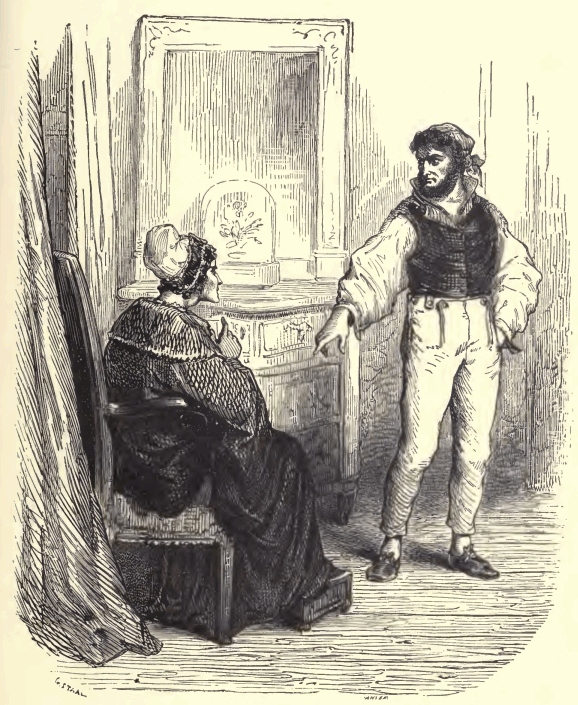
\includegraphics[width=\textwidth]{0323m.jpg}
\end{figure}

Like other dwellers in the south, he was a man of sober habits and
moderate desires, but fond of external show, vain, and addicted to
display. During the days of his prosperity, not a festivity took place
without himself and wife being among the spectators. He dressed in the
picturesque costume worn upon grand occasions by the inhabitants of the
south of France, bearing equal resemblance to the style adopted both by
the Catalans and Andalusians; while La Carconte displayed the charming
fashion prevalent among the women of Arles, a mode of attire borrowed
equally from Greece and Arabia. But, by degrees, watch-chains,
necklaces, parti-colored scarves, embroidered bodices, velvet vests,
elegantly worked stockings, striped gaiters, and silver buckles for the
shoes, all disappeared; and Gaspard Caderousse, unable to appear abroad
in his pristine splendor, had given up any further participation in the
pomps and vanities, both for himself and wife, although a bitter
feeling of envious discontent filled his mind as the sound of mirth and
merry music from the joyous revellers reached even the miserable
hostelry to which he still clung, more for the shelter than the profit
it afforded.

Caderousse, then, was, as usual, at his place of observation before the
door, his eyes glancing listlessly from a piece of closely shaven
grass—on which some fowls were industriously, though fruitlessly,
endeavoring to turn up some grain or insect suited to their palate—to
the deserted road, which led away to the north and south, when he was
aroused by the shrill voice of his wife, and grumbling to himself as he
went, he mounted to her chamber, first taking care, however, to set the
entrance door wide open, as an invitation to any chance traveller who
might be passing.

At the moment Caderousse quitted his sentry-like watch before the door,
the road on which he so eagerly strained his sight was void and lonely
as a desert at midday. There it lay stretching out into one
interminable line of dust and sand, with its sides bordered by tall,
meagre trees, altogether presenting so uninviting an appearance, that
no one in his senses could have imagined that any traveller, at liberty
to regulate his hours for journeying, would choose to expose himself in
such a formidable Sahara.

Nevertheless, had Caderousse but retained his post a few minutes
longer, he might have caught a dim outline of something approaching
from the direction of Bellegarde; as the moving object drew nearer, he
would easily have perceived that it consisted of a man and horse,
between whom the kindest and most amiable understanding appeared to
exist. The horse was of Hungarian breed, and ambled along at an easy
pace. His rider was a priest, dressed in black, and wearing a
three-cornered hat; and, spite of the ardent rays of a noonday sun, the
pair came on with a fair degree of rapidity.

Having arrived before the Pont du Gard, the horse stopped, but whether
for his own pleasure or that of his rider would have been difficult to
say. However that might have been, the priest, dismounting, led his
steed by the bridle in search of some place to which he could secure
him. Availing himself of a handle that projected from a half-fallen
door, he tied the animal safely and having drawn a red cotton
handkerchief, from his pocket, wiped away the perspiration that
streamed from his brow, then, advancing to the door, struck thrice with
the end of his iron-shod stick.

At this unusual sound, a huge black dog came rushing to meet the daring
assailant of his ordinarily tranquil abode, snarling and displaying his
sharp white teeth with a determined hostility that abundantly proved
how little he was accustomed to society. At that moment a heavy
footstep was heard descending the wooden staircase that led from the
upper floor, and, with many bows and courteous smiles, the host of the
Pont du Gard besought his guest to enter.

\begin{figure}[h]
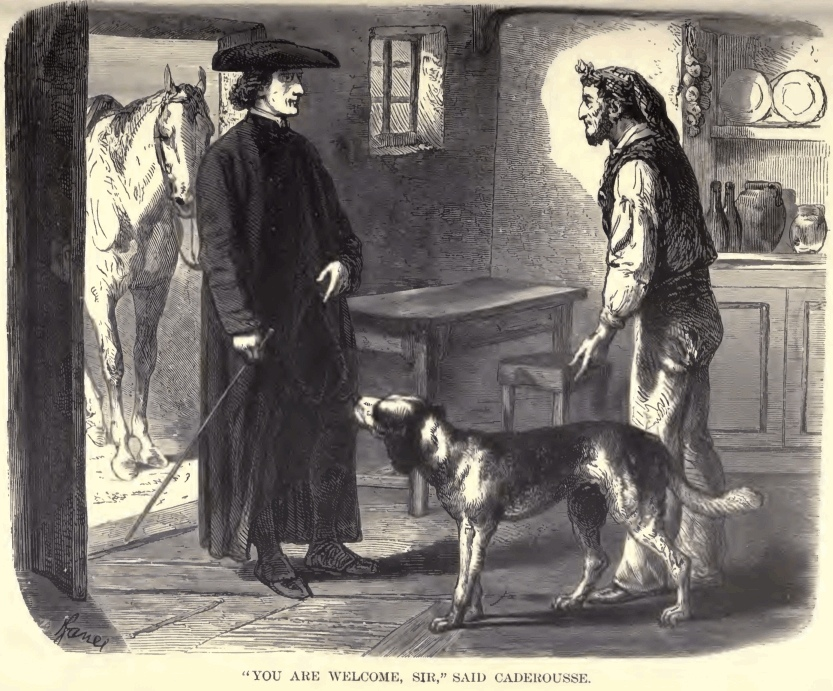
\includegraphics[width=\textwidth]{0319m.jpg}
\end{figure}

“You are welcome, sir, most welcome!” repeated the astonished
Caderousse. “Now, then, Margotin,” cried he, speaking to the dog, “will
you be quiet? Pray don’t heed him, sir!—he only barks, he never bites.
I make no doubt a glass of good wine would be acceptable this
dreadfully hot day.” Then perceiving for the first time the garb of the
traveller he had to entertain, Caderousse hastily exclaimed: “A
thousand pardons! I really did not observe whom I had the honor to
receive under my poor roof. What would the abbé please to have? What
refreshment can I offer? All I have is at his service.”

The priest gazed on the person addressing him with a long and searching
gaze—there even seemed a disposition on his part to court a similar
scrutiny on the part of the innkeeper; then, observing in the
countenance of the latter no other expression than extreme surprise at
his own want of attention to an inquiry so courteously worded, he
deemed it as well to terminate this dumb show, and therefore said,
speaking with a strong Italian accent, “You are, I presume, M.
Caderousse?”

“Yes, sir,” answered the host, even more surprised at the question than
he had been by the silence which had preceded it; “I am Gaspard
Caderousse, at your service.”

“Gaspard Caderousse,” rejoined the priest. “Yes,— Christian and surname
are the same. You formerly lived, I believe in the Allées de Meilhan,
on the fourth floor?”

\begin{figure}[ht]
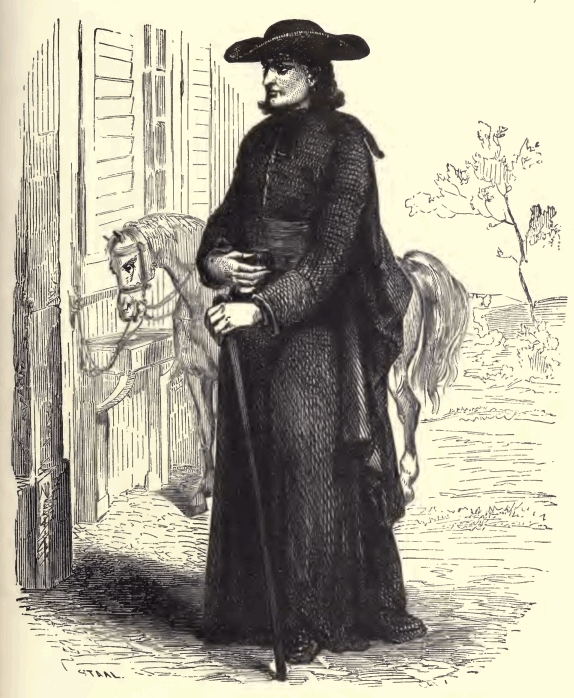
\includegraphics[width=\textwidth]{0325m.jpg}
\end{figure}

“I did.”

“And you followed the business of a tailor?”

“True, I was a tailor, till the trade fell off. It is so hot at
Marseilles, that really I believe that the respectable inhabitants will
in time go without any clothing whatever. But talking of heat, is there
nothing I can offer you by way of refreshment?”

“Yes; let me have a bottle of your best wine, and then, with your
permission, we will resume our conversation from where we left off.”

“As you please, sir,” said Caderousse, who, anxious not to lose the
present opportunity of finding a customer for one of the few bottles of
Cahors still remaining in his possession, hastily raised a trap-door in
the floor of the apartment they were in, which served both as parlor
and kitchen.

Upon issuing forth from his subterranean retreat at the expiration of
five minutes, he found the abbé seated upon a wooden stool, leaning his
elbow on a table, while Margotin, whose animosity seemed appeased by
the unusual command of the traveller for refreshments, had crept up to
him, and had established himself very comfortably between his knees,
his long, skinny neck resting on his lap, while his dim eye was fixed
earnestly on the traveller’s face.

“Are you quite alone?” inquired the guest, as Caderousse placed before
him the bottle of wine and a glass.

“Quite, quite alone,” replied the man—“or, at least, practically so,
for my poor wife, who is the only person in the house besides myself,
is laid up with illness, and unable to render me the least assistance,
poor thing!”

“You are married, then?” said the priest, with a show of interest,
glancing round as he spoke at the scanty furnishings of the apartment.

“Ah, sir,” said Caderousse with a sigh, “it is easy to perceive I am
not a rich man; but in this world a man does not thrive the better for
being honest.” The abbé fixed on him a searching, penetrating glance.

“Yes, honest—I can certainly say that much for myself,” continued the
innkeeper, fairly sustaining the scrutiny of the abbé’s gaze; “I can
boast with truth of being an honest man; and,” continued he
significantly, with a hand on his breast and shaking his head, “that is
more than everyone can say nowadays.”

\begin{figure}[ht]
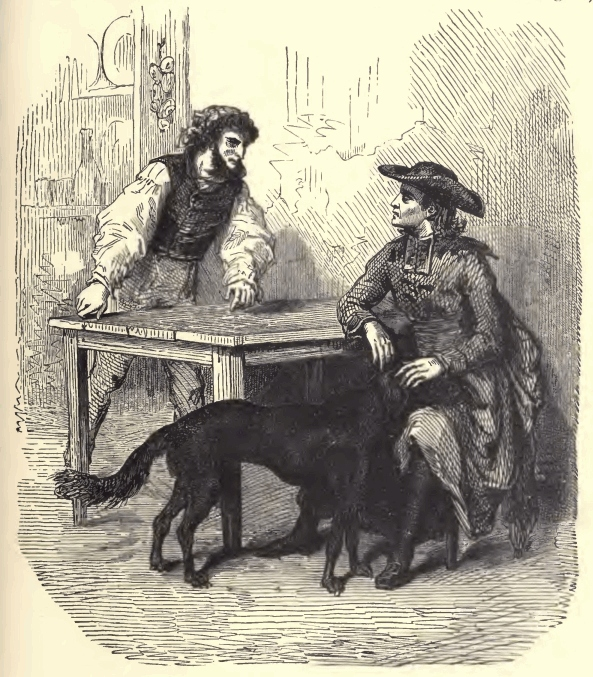
\includegraphics[width=\textwidth]{0327m.jpg}
\end{figure}

“So much the better for you, if what you assert be true,” said the
abbé; “for I am firmly persuaded that, sooner or later, the good will
be rewarded, and the wicked punished.”

“Such words as those belong to your profession,” answered Caderousse,
“and you do well to repeat them; but,” added he, with a bitter
expression of countenance, “one is free to believe them or not, as one
pleases.”

“You are wrong to speak thus,” said the abbé; “and perhaps I may, in my
own person, be able to prove to you how completely you are in error.”

“What mean you?” inquired Caderousse with a look of surprise.

“In the first place, I must be satisfied that you are the person I am
in search of.”

“What proofs do you require?”

“Did you, in the year 1814 or 1815, know anything of a young sailor
named Dantès?”

“Dantès? Did I know poor dear Edmond? Why, Edmond Dantès and myself
were intimate friends!” exclaimed Caderousse, whose countenance flushed
darkly as he caught the penetrating gaze of the abbé fixed on him,
while the clear, calm eye of the questioner seemed to dilate with
feverish scrutiny.

“You remind me,” said the priest, “that the young man concerning whom I
asked you was said to bear the name of Edmond.”

“Said to bear the name!” repeated Caderousse, becoming excited and
eager. “Why, he was so called as truly as I myself bore the appellation
of Gaspard Caderousse; but tell me, I pray, what has become of poor
Edmond? Did you know him? Is he alive and at liberty? Is he prosperous
and happy?”

“He died a more wretched, hopeless, heart-broken prisoner than the
felons who pay the penalty of their crimes at the galleys of Toulon.”

A deadly pallor followed the flush on the countenance of Caderousse,
who turned away, and the priest saw him wiping the tears from his eyes
with the corner of the red handkerchief twisted round his head.

“Poor fellow, poor fellow!” murmured Caderousse. “Well, there, sir, is
another proof that good people are never rewarded on this earth, and
that none but the wicked prosper. Ah,” continued Caderousse, speaking
in the highly colored language of the South, “the world grows worse and
worse. Why does not God, if he really hates the wicked, as he is said
to do, send down brimstone and fire, and consume them altogether?”

“You speak as though you had loved this young Dantès,” observed the
abbé, without taking any notice of his companion’s vehemence.

“And so I did,” replied Caderousse; “though once, I confess, I envied
him his good fortune. But I swear to you, sir, I swear to you, by
everything a man holds dear, I have, since then, deeply and sincerely
lamented his unhappy fate.”

There was a brief silence, during which the fixed, searching eye of the
abbé was employed in scrutinizing the agitated features of the
innkeeper.

“You knew the poor lad, then?” continued Caderousse.

“I was called to see him on his dying bed, that I might administer to
him the consolations of religion.”

“And of what did he die?” asked Caderousse in a choking voice.

“Of what, think you, do young and strong men die in prison, when they
have scarcely numbered their thirtieth year, unless it be of
imprisonment?” Caderousse wiped away the large beads of perspiration
that gathered on his brow.

\begin{figure}[h]
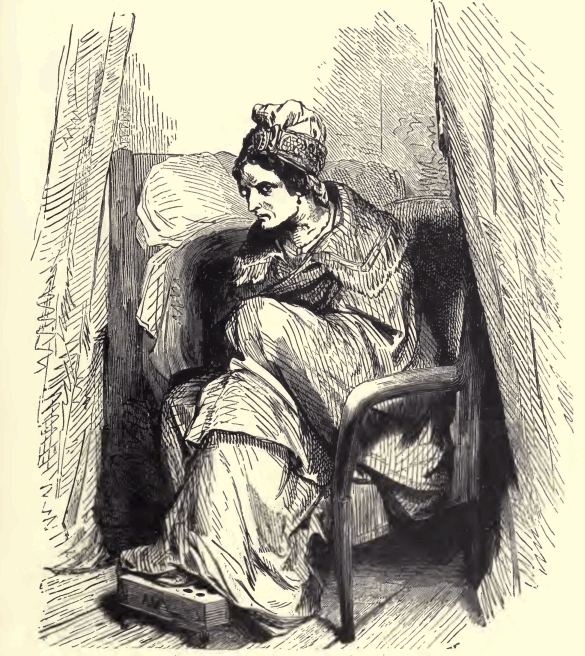
\includegraphics[width=\textwidth]{0329m.jpg}
\end{figure}

“But the strangest part of the story is,” resumed the abbé, “that
Dantès, even in his dying moments, swore by his crucified Redeemer,
that he was utterly ignorant of the cause of his detention.”

“And so he was,” murmured Caderousse. “How should he have been
otherwise? Ah, sir, the poor fellow told you the truth.”

“And for that reason, he besought me to try and clear up a mystery he
had never been able to penetrate, and to clear his memory should any
foul spot or stain have fallen on it.”

And here the look of the abbé, becoming more and more fixed, seemed to
rest with ill-concealed satisfaction on the gloomy depression which was
rapidly spreading over the countenance of Caderousse.

“A rich Englishman,” continued the abbé, “who had been his companion in
misfortune, but had been released from prison during the second
restoration, was possessed of a diamond of immense value; this jewel he
bestowed on Dantès upon himself quitting the prison, as a mark of his
gratitude for the kindness and brotherly care with which Dantès had
nursed him in a severe illness he underwent during his confinement.
Instead of employing this diamond in attempting to bribe his jailers,
who might only have taken it and then betrayed him to the governor,
Dantès carefully preserved it, that in the event of his getting out of
prison he might have wherewithal to live, for the sale of such a
diamond would have quite sufficed to make his fortune.”

“Then, I suppose,” asked Caderousse, with eager, glowing looks, “that
it was a stone of immense value?”

“Why, everything is relative,” answered the abbé. “To one in Edmond’s
position the diamond certainly was of great value. It was estimated at
fifty thousand francs.”

“Bless me!” exclaimed Caderousse, “fifty thousand francs! Surely the
diamond was as large as a nut to be worth all that.”

“No,” replied the abbé, “it was not of such a size as that; but you
shall judge for yourself. I have it with me.”

The sharp gaze of Caderousse was instantly directed towards the
priest’s garments, as though hoping to discover the location of the
treasure. Calmly drawing forth from his pocket a small box covered with
black shagreen, the abbé opened it, and displayed to the dazzled eyes
of Caderousse the sparkling jewel it contained, set in a ring of
admirable workmanship.

“And that diamond,” cried Caderousse, almost breathless with eager
admiration, “you say, is worth fifty thousand francs?”

“It is, without the setting, which is also valuable,” replied the abbé,
as he closed the box, and returned it to his pocket, while its
brilliant hues seemed still to dance before the eyes of the fascinated
innkeeper.

“But how comes the diamond in your possession, sir? Did Edmond make you
his heir?”

“No, merely his testamentary executor. ‘I once possessed four dear and
faithful friends, besides the maiden to whom I was betrothed’ he said;
‘and I feel convinced they have all unfeignedly grieved over my loss.
The name of one of the four friends is Caderousse.’” The innkeeper
shivered.

“‘Another of the number,’” continued the abbé, without seeming to
notice the emotion of Caderousse, “‘is called Danglars; and the third,
in spite of being my rival, entertained a very sincere affection for
me.’”

A fiendish smile played over the features of Caderousse, who was about
to break in upon the abbé’s speech, when the latter, waving his hand,
said, “Allow me to finish first, and then if you have any observations
to make, you can do so afterwards. ‘The third of my friends, although
my rival, was much attached to me,—his name was Fernand; that of my
betrothed was’—Stay, stay,” continued the abbé, “I have forgotten what
he called her.”

“Mercédès,” said Caderousse eagerly.

“True,” said the abbé, with a stifled sigh, “Mercédès it was.”

“Go on,” urged Caderousse.

“Bring me a \textit{carafe} of water,” said the abbé.

Caderousse quickly performed the stranger’s bidding; and after pouring
some into a glass, and slowly swallowing its contents, the abbé,
resuming his usual placidity of manner, said, as he placed his empty
glass on the table:

“Where did we leave off?”

“The name of Edmond’s betrothed was Mercédès.”

“To be sure. ‘You will go to Marseilles,’ said Dantès,—for you
understand, I repeat his words just as he uttered them. Do you
understand?”

“Perfectly.”

“‘You will sell this diamond; you will divide the money into five equal
parts, and give an equal portion to these good friends, the only
persons who have loved me upon earth.’”

“But why into five parts?” asked Caderousse; “you only mentioned four
persons.”

“Because the fifth is dead, as I hear. The fifth sharer in Edmond’s
bequest, was his own father.”

“Too true, too true!” ejaculated Caderousse, almost suffocated by the
contending passions which assailed him, “the poor old man did die.”

“I learned so much at Marseilles,” replied the abbé, making a strong
effort to appear indifferent; “but from the length of time that has
elapsed since the death of the elder Dantès, I was unable to obtain any
particulars of his end. Can you enlighten me on that point?”

“I do not know who could if I could not,” said Caderousse. “Why, I
lived almost on the same floor with the poor old man. Ah, yes, about a
year after the disappearance of his son the poor old man died.”

“Of what did he die?”

“Why, the doctors called his complaint gastro-enteritis, I believe; his
acquaintances say he died of grief; but I, who saw him in his dying
moments, I say he died of——”

Caderousse paused.

“Of what?” asked the priest, anxiously and eagerly.

“Why, of downright starvation.”

“Starvation!” exclaimed the abbé, springing from his seat. “Why, the
vilest animals are not suffered to die by such a death as that. The
very dogs that wander houseless and homeless in the streets find some
pitying hand to cast them a mouthful of bread; and that a man, a
Christian, should be allowed to perish of hunger in the midst of other
men who call themselves Christians, is too horrible for belief. Oh, it
is impossible!—utterly impossible!”

“What I have said, I have said,” answered Caderousse.

“And you are a fool for having said anything about it,” said a voice
from the top of the stairs. “Why should you meddle with what does not
concern you?”

The two men turned quickly, and saw the sickly countenance of La
Carconte peering between the baluster rails; attracted by the sound of
voices, she had feebly dragged herself down the stairs, and, seated on
the lower step, head on knees, she had listened to the foregoing
conversation.

“Mind your own business, wife,” replied Caderousse sharply. “This
gentleman asks me for information, which common politeness will not
permit me to refuse.”

“Politeness, you simpleton!” retorted La Carconte. “What have you to do
with politeness, I should like to know? Better study a little common
prudence. How do you know the motives that person may have for trying
to extract all he can from you?”

“I pledge you my word, madam,” said the abbé, “that my intentions are
good; and that your husband can incur no risk, provided he answers me
candidly.”

“Ah, that’s all very fine,” retorted the woman. “Nothing is easier than
to begin with fair promises and assurances of nothing to fear; but when
poor, silly folks, like my husband there, have been persuaded to tell
all they know, the promises and assurances of safety are quickly
forgotten; and at some moment when nobody is expecting it, behold
trouble and misery, and all sorts of persecutions, are heaped on the
unfortunate wretches, who cannot even see whence all their afflictions
come.”

“Nay, nay, my good woman, make yourself perfectly easy, I beg of you.
Whatever evils may befall you, they will not be occasioned by my
instrumentality, that I solemnly promise you.”

La Carconte muttered a few inarticulate words, then let her head again
drop upon her knees, and went into a fit of ague, leaving the two
speakers to resume the conversation, but remaining so as to be able to
hear every word they uttered. Again the abbé had been obliged to
swallow a draught of water to calm the emotions that threatened to
overpower him.

When he had sufficiently recovered himself, he said, “It appears, then,
that the miserable old man you were telling me of was forsaken by
everyone. Surely, had not such been the case, he would not have
perished by so dreadful a death.”

“Why, he was not altogether forsaken,” continued Caderousse, “for
Mercédès the Catalan and Monsieur Morrel were very kind to him; but
somehow the poor old man had contracted a profound hatred for
Fernand—the very person,” added Caderousse with a bitter smile, “that
you named just now as being one of Dantès’ faithful and attached
friends.”

“And was he not so?” asked the abbé.

“Gaspard, Gaspard!” murmured the woman, from her seat on the stairs,
“mind what you are saying!”

Caderousse made no reply to these words, though evidently irritated and
annoyed by the interruption, but, addressing the abbé, said, “Can a man
be faithful to another whose wife he covets and desires for himself?
But Dantès was so honorable and true in his own nature, that he
believed everybody’s professions of friendship. Poor Edmond, he was
cruelly deceived; but it was fortunate that he never knew, or he might
have found it more difficult, when on his deathbed, to pardon his
enemies. And, whatever people may say,” continued Caderousse, in his
native language, which was not altogether devoid of rude poetry, “I
cannot help being more frightened at the idea of the malediction of the
dead than the hatred of the living.”

“Imbecile!” exclaimed La Carconte.

“Do you, then, know in what manner Fernand injured Dantès?” inquired
the abbé of Caderousse.

“Do I? No one better.”

“Speak out then, say what it was!”

“Gaspard!” cried La Carconte, “do as you will; you are master—but if
you take my advice you’ll hold your tongue.”

“Well, wife,” replied Caderousse, “I don’t know but what you’re right!”

“So you will say nothing?” asked the abbé.

“Why, what good would it do?” asked Caderousse. “If the poor lad were
living, and came to me and begged that I would candidly tell which were
his true and which his false friends, why, perhaps, I should not
hesitate. But you tell me he is no more, and therefore can have nothing
to do with hatred or revenge, so let all such feeling be buried with
him.”

“You prefer, then,” said the abbé, “that I should bestow on men you say
are false and treacherous, the reward intended for faithful
friendship?”

“That is true enough,” returned Caderousse. “You say truly, the gift of
poor Edmond was not meant for such traitors as Fernand and Danglars;
besides, what would it be to them? no more than a drop of water in the
ocean.”

“Remember,” chimed in La Carconte, “those two could crush you at a
single blow!”

“How so?” inquired the abbé. “Are these persons, then, so rich and
powerful?”

“Do you not know their history?”

“I do not. Pray relate it to me!”

Caderousse seemed to reflect for a few moments, then said, “No, truly,
it would take up too much time.”

“Well, my good friend,” returned the abbé, in a tone that indicated
utter indifference on his part, “you are at liberty, either to speak or
be silent, just as you please; for my own part, I respect your scruples
and admire your sentiments; so let the matter end. I shall do my duty
as conscientiously as I can, and fulfil my promise to the dying man. My
first business will be to dispose of this diamond.”

So saying, the abbé again drew the small box from his pocket, opened
it, and contrived to hold it in such a light, that a bright flash of
brilliant hues passed before the dazzled gaze of Caderousse.

“Wife, wife!” cried he in a hoarse voice, “come here!”

“Diamond!” exclaimed La Carconte, rising and descending to the chamber
with a tolerably firm step; “what diamond are you talking about?”

“Why, did you not hear all we said?” inquired Caderousse. “It is a
beautiful diamond left by poor Edmond Dantès, to be sold, and the money
divided between his father, Mercédès, his betrothed bride, Fernand,
Danglars, and myself. The jewel is worth at least fifty thousand
francs.”

“Oh, what a magnificent jewel!” cried the astonished woman.

“The fifth part of the profits from this stone belongs to us then, does
it not?” asked Caderousse.

“It does,” replied the abbé; “with the addition of an equal division of
that part intended for the elder Dantès, which I believe myself at
liberty to divide equally with the four survivors.”

“And why among us four?” inquired Caderousse.

“As being the friends Edmond esteemed most faithful and devoted to
him.”

“I don’t call those friends who betray and ruin you,” murmured the wife
in her turn, in a low, muttering voice.

“Of course not!” rejoined Caderousse quickly; “no more do I, and that
was what I was observing to this gentleman just now. I said I looked
upon it as a sacrilegious profanation to reward treachery, perhaps
crime.”

“Remember,” answered the abbé calmly, as he replaced the jewel and its
case in the pocket of his cassock, “it is your fault, not mine, that I
do so. You will have the goodness to furnish me with the address of
both Fernand and Danglars, in order that I may execute Edmond’s last
wishes.”

The agitation of Caderousse became extreme, and large drops of
perspiration rolled from his heated brow. As he saw the abbé rise from
his seat and go towards the door, as though to ascertain if his horse
were sufficiently refreshed to continue his journey, Caderousse and his
wife exchanged looks of deep meaning.

\begin{figure}[ht]
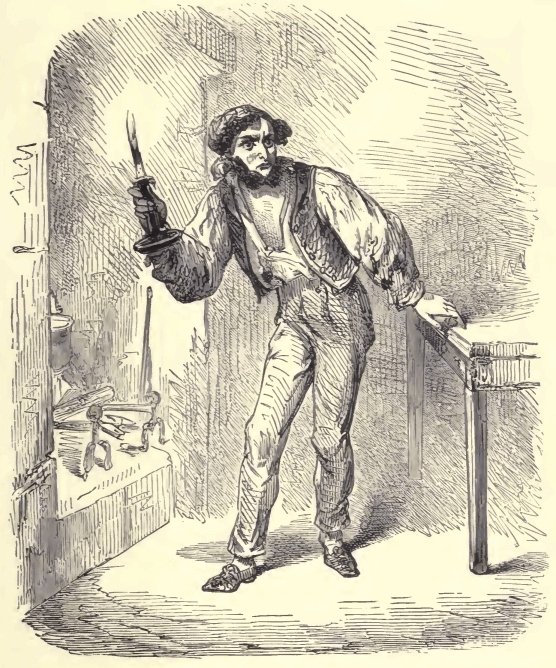
\includegraphics[width=\textwidth]{0335m.jpg}
\end{figure}

“There, you see, wife,” said the former, “this splendid diamond might
all be ours, if we chose!”

“Do you believe it?”

“Why, surely a man of his holy profession would not deceive us!”

“Well,” replied La Carconte, “do as you like. For my part, I wash my
hands of the affair.”

So saying, she once more climbed the staircase leading to her chamber,
her body convulsed with chills, and her teeth rattling in her head, in
spite of the intense heat of the weather. Arrived at the top stair, she
turned round, and called out, in a warning tone, to her husband,
“Gaspard, consider well what you are about to do!”

“I have both reflected and decided,” answered he.

La Carconte then entered her chamber, the flooring of which creaked
beneath her heavy, uncertain tread, as she proceeded towards her
armchair, into which she fell as though exhausted.

“Well,” asked the abbé, as he returned to the apartment below, “what
have you made up your mind to do?”

“To tell you all I know,” was the reply.

“I certainly think you act wisely in so doing,” said the priest. “Not
because I have the least desire to learn anything you may please to
conceal from me, but simply that if, through your assistance, I could
distribute the legacy according to the wishes of the testator, why, so
much the better, that is all.”

“I hope it may be so,” replied Caderousse, his face flushed with
cupidity.

“I am all attention,” said the abbé.

“Stop a minute,” answered Caderousse; “we might be interrupted in the
most interesting part of my story, which would be a pity; and it is as
well that your visit hither should be made known only to ourselves.”

With these words he went stealthily to the door, which he closed, and,
by way of still greater precaution, bolted and barred it, as he was
accustomed to do at night.

During this time the abbé had chosen his place for listening at his
ease. He removed his seat into a corner of the room, where he himself
would be in deep shadow, while the light would be fully thrown on the
narrator; then, with head bent down and hands clasped, or rather
clenched together, he prepared to give his whole attention to
Caderousse, who seated himself on the little stool, exactly opposite to
him.

“Remember, this is no affair of mine,” said the trembling voice of La
Carconte, as though through the flooring of her chamber she viewed the
scene that was enacting below.

“Enough, enough!” replied Caderousse; “say no more about it; I will
take all the consequences upon myself.”

And he began his story.
